%% 
%% Copyright 2007-2026 Elsevier Ltd
%% 
%% This file is part of the 'Elsarticle Bundle'.
%% ---------------------------------------------
%% 
%% It may be distributed under the conditions of the LaTeX Project Public
%% License, either version 1.3 of this license or (at your option) any
%% later version.  The latest version of this license is in
%%    http://www.latex-project.org/lppl.txt
%% and version 1.3 or later is part of all distributions of LaTeX
%% version 1999/12/01 or later.
%% 
%% The list of all files belonging to the 'Elsarticle Bundle' is
%% given in the file `manifest.txt'.
%% 
%% Template article for Elsevier's document class `elsarticle'
%% with numbered style bibliographic references
%% SP 2008/03/01
%% $Id: elsarticle-template-num.tex 289 2026-01-09 06:13:01Z rishi $
%%
\documentclass[preprint,12pt]{elsarticle}

%% Use the option review to obtain double line spacing
%% \documentclass[authoryear,preprint,review,12pt]{elsarticle}

%% Use the options 1p,twocolumn; 3p; 3p,twocolumn; 5p; or 5p,twocolumn
%% for a journal layout:
%% \documentclass[final,1p,times]{elsarticle}
%% \documentclass[final,1p,times,twocolumn]{elsarticle}
%% \documentclass[final,3p,times]{elsarticle}
%% \documentclass[final,3p,times,twocolumn]{elsarticle}
%% \documentclass[final,5p,times]{elsarticle}
%% \documentclass[final,5p,times,twocolumn]{elsarticle}

%% For including figures, graphicx.sty has been loaded in
%% elsarticle.cls. If you prefer to use the old commands
%% please give \usepackage{epsfig}

%% The amssymb package provides various useful mathematical symbols
\usepackage{amssymb}
%% The amsmath package provides various useful equation environments.
\usepackage{amsmath}
%% booktabs gives cleaner \toprule/\midrule/\bottomrule table rules
\usepackage{booktabs}
%% tikz draws the architecture and sampling-mechanism diagrams as vector
%% graphics directly in the source, rather than external image files.
\usepackage{tikz}
\usetikzlibrary{arrows.meta,positioning,fit,backgrounds,decorations.pathreplacing,calc}
\usepackage{graphicx}
%% The generated .bbl defines \path as a trivial passthrough (which
%% breaks on a bare underscore in a DOI, outside math mode) unless
%% \href is already defined when the .bbl is read; \providecommand
%% here short-circuits that fallback, then \path is aliased to \url
%% (from the url package) for its underscore-safe catcode handling.
\usepackage{url}
\providecommand{\href}[2]{#2}
\let\path\url
%% The amsthm package provides extended theorem environments
%% \usepackage{amsthm}

%% The lineno packages adds line numbers. Start line numbering with
%% \begin{linenumbers}, end it with \end{linenumbers}. Or switch it on
%% for the whole article with \linenumbers.
%% \usepackage{lineno}

\journal{Computer Methods and Programs in Biomedicine}

\begin{document}

\begin{frontmatter}

%% Title, authors and addresses

%% use the tnoteref command within \title for footnotes;
%% use the tnotetext command for theassociated footnote;
%% use the fnref command within \author or \affiliation for footnotes;
%% use the fntext command for theassociated footnote;
%% use the corref command within \author for corresponding author footnotes;
%% use the cortext command for theassociated footnote;
%% use the ead command for the email address,
%% and the form \ead[url] for the home page:
%% \title{Title\tnoteref{label1}}
%% \tnotetext[label1]{}
%% \author{Name\corref{cor1}\fnref{label2}}
%% \ead{email address}
%% \ead[url]{home page}
%% \fntext[label2]{}
%% \cortext[cor1]{}
%% \affiliation{organization={},
%%             addressline={},
%%             city={},
%%             postcode={},
%%             state={},
%%             country={}}
%% \fntext[label3]{}

\title{Efficient Frame Sampling for Surgical Phase Recognition: A Compute-Aware Hybrid Sampler Informed by Systematic Ablation}

%% use optional labels to link authors explicitly to addresses:
%% \author[label1,label2]{}
%% \affiliation[label1]{organization={},
%%             addressline={},
%%             city={},
%%             postcode={},
%%             state={},
%%             country={}}
%%
%% \affiliation[label2]{organization={},
%%             addressline={},
%%             city={},
%%             postcode={},
%%             state={},
%%             country={}}

\author[1]{Luning Li}
\author[2]{Yohei Sanmoto}
\author[3]{Yudai Goto}
\author[4]{Xuhan Zhu}
\author[1]{Xin Zhu\corref{cor1}}
\ead{zhu.xin@tmd.ac.jp}
\cortext[cor1]{Corresponding author.}

%% Author affiliations
\affiliation[1]{organization={Department of AI Technology Development, M\&D Data Science Center, Institute of Biomedical Engineering, Institute of Science Tokyo},
            city={Tokyo},
            country={Japan}}
\affiliation[2]{organization={University of Tsukuba},
            city={Tsukuba},
            country={Japan}}
\affiliation[3]{organization={University of Tsukuba Hospital},
            city={Tsukuba},
            country={Japan}}
\affiliation[4]{organization={Graduate School of Medical and Dental Sciences, Institute of Science Tokyo},
            city={Tokyo},
            country={Japan}}

%% Abstract
\begin{abstract}
%% Text of abstract
\textbf{Background and Objective:} Surgical phase recognition pipelines commonly process every frame in a temporal window despite substantial visual redundancy in laparoscopic video. Learned key-frame selection is widely assumed to reduce computation while preserving or improving accuracy, but this assumption is rarely tested against a simple non-learned baseline.

\textbf{Methods:} We systematically evaluate ten jointly-trained frame-scoring architectures, plain uniform pooling, and stochastic per-step random resampling on Cholec80, using three downstream classifiers (BiGRU, TeCNO, Trans-SVNet). We derive a closed-form entropy account of the resampling effect and reproduce two published sampling methods (MGSampler, SCSampler) under matched evaluation. Guided by this diagnosis, we propose MobileNet-TS+, a lightweight pixel-level sampler jointly supervised on phase label and optical-flow regression, deployed via a training/inference-decoupled recipe.

\textbf{Results:} All ten learned scorers underperform plain uniform pooling (macro-Jaccard 0.65--0.68 vs.\ 0.71--0.73); per-step random resampling instead reaches 0.7466, attributable to injected training-time entropy rather than frame quality. MobileNet-TS+ reaches 0.7543 under deterministic deployment, within 0.22 points of an uncompressed accuracy ceiling that forgoes all compute savings, while retaining a 48.5\% reduction in ViT-encoder FLOPs. Across a 324-configuration sweep spanning three datasets (Cholec80, AutoLaparo, HeiChole), three architectures (BiGRU, TeCNO, Trans-SVNet, all trained under a uniform crossover recipe found to match or exceed native training for every architecture), this advantage is small but statistically significant overall ($p=0.0060$), and concentrates specifically at moderate sampling granularity (bin\_size=8) rather than being cleanly predicted by architecture regularization or dataset scale alone.

\textbf{Conclusion:} Learned importance sampling is not inherently beneficial for surgical phase recognition; its value is conditional on sampling granularity and on whether the deployment can spare full per-frame encoding at all, rather than on downstream architecture or data scale alone. MobileNet-TS+ offers a diagnosis-driven, compute-efficient alternative that improves on non-learned sampling while retaining most of the encoder-compute savings that motivate frame selection in the first place; a substantially higher accuracy ceiling remains reachable only by giving up those savings entirely.
\end{abstract}

%%Graphical abstract
\begin{graphicalabstract}
\centering
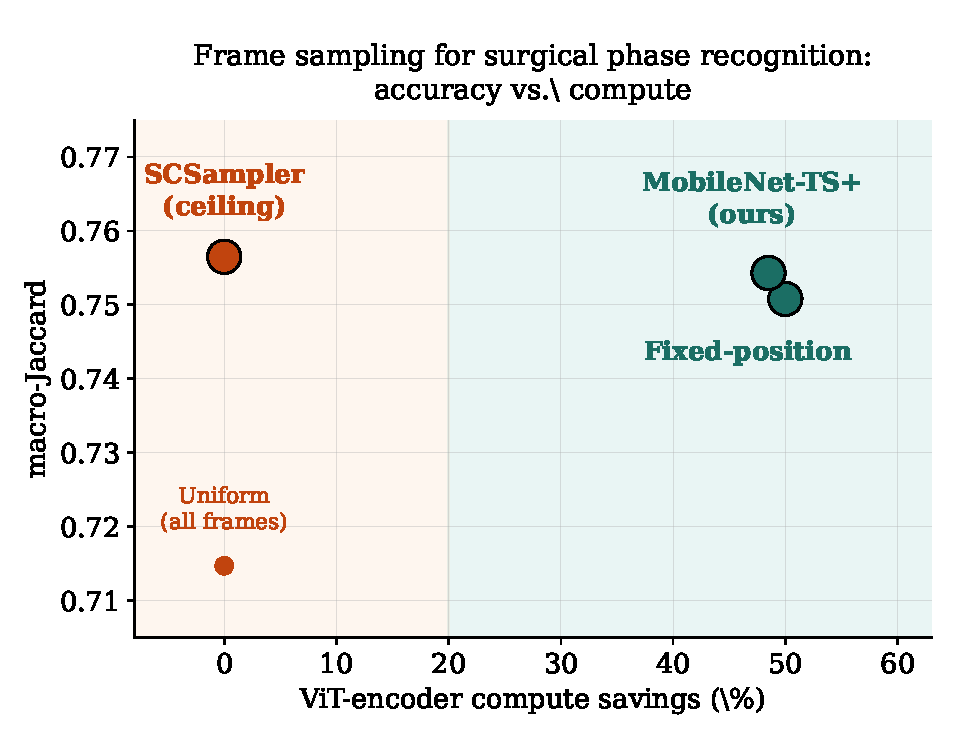
\includegraphics[width=0.7\linewidth]{figures/graphical_abstract.pdf}
\end{graphicalabstract}

%%Research highlights
\begin{highlights}
\item Learned frame samplers fail to beat random resampling on surgical phase recognition.
\item The benefit comes from training-time entropy, not from selecting better frames.
\item MobileNet-TS+ gives a small, validated accuracy gain over Fixed-position while nearly halving ViT-encoder compute; closing the remaining gap to an uncompressed accuracy ceiling requires giving up those compute savings entirely.
\item Validated across 324 configurations (3 datasets, 3 architectures, full window/top\_k sweep).
\item A crossover training recipe (random resampling in training, the learned rule at inference) matches or beats native training for every architecture tested, including those with strong built-in regularization.
\end{highlights}

%% Keywords
\begin{keyword}
surgical phase recognition \sep frame sampling \sep temporal redundancy \sep efficient video understanding \sep Cholec80

%% PACS codes here, in the form: \PACS code \sep code

%% MSC codes here, in the form: \MSC code \sep code
%% or \MSC[2008] code \sep code (2000 is the default)

\end{keyword}

\end{frontmatter}

%% Add \usepackage{lineno} before \begin{document} and uncomment 
%% following line to enable line numbers
%% \linenumbers

%% main text
%%

\section{Introduction}
\label{sec:intro}

%% [中文] 段1 背景 + 效率瓶颈: 交代手术阶段识别的应用背景，指出一台
%% 腹腔镜手术产生上千帧、相邻帧高度冗余，导致每帧都过一遍大模型编码器
%% 很浪费算力。这段负责建立"为什么要做帧采样"这个问题本身。
Surgical phase recognition -- the task of identifying which stage of a procedure is depicted in a given segment of intraoperative video -- underpins downstream applications such as workflow monitoring, resource scheduling, skill assessment, and context-aware assistance systems~\cite{czempiel2020tecno}. A laparoscopic cholecystectomy typically spans 30--90 minutes; even sampled at 1 frame per second, a single procedure yields thousands of frames, many of which are visually near-identical. During steady dissection or camera holds, consecutive frames differ only marginally, so processing every frame with a modern encoder (a Vision Transformer or comparable backbone) spends the majority of its computation on frames that are individually redundant with their neighbors.

%% [中文] 段2 现有范式的默认假设: 介绍高效帧采样的两条主流路线——
%% MGSampler(运动引导，确定性)和SCSampler(学习式打分)，两者在通用
%% 视频领域都报告了明显提升。点出两者背后共同的隐含假设："选有信息量
%% 的帧，比全部池化或随便选，更好"。这段负责交代"大家默认相信什么"。
This observation has motivated a body of work on \emph{efficient frame sampling}: rather than encoding every frame in a temporal window, a lightweight mechanism selects an informative subset before the expensive encoder is invoked. In general video understanding, this idea has taken two dominant forms. Motion-guided samplers such as MGSampler~\cite{zhi2021mgsampler} place samples according to a cumulative motion distribution, favoring temporally denser sampling where visual change is concentrated. Learned-saliency samplers such as SCSampler~\cite{korbar2019scsampler} instead train a lightweight scorer to predict how useful a candidate clip will be to the downstream recognition model, and retain only the highest-scoring candidates. Both report substantial accuracy and/or efficiency gains over naive uniform sampling on large-scale, general-domain action recognition benchmarks. The implicit assumption underlying both lines of work -- and, more broadly, underlying the common practice of building a learned selector whenever a task exhibits input redundancy -- is that \emph{choosing informative frames is better than pooling all of them, or than choosing arbitrarily}.

%% [中文] 段3 假设为什么没被真正测过 (本文要填补的gap): 指出手术视频
%% 和通用视频领域的两个关键差异——① 公开手术数据集比通用视频语料小
%% 1-2个数量级；② 下游分类器从"几乎没有内置时序正则化"到"自带很强
%% 正则化"跨度很大。这个假设在这种规模/架构下是否还成立，此前没人
%% 系统测过——这段负责建立"gap"。
Surgical video departs from the general-domain setting these methods were developed on in two respects that are rarely tested explicitly: publicly available surgical datasets are one to two orders of magnitude smaller than the video corpora used to validate general-purpose samplers, and the downstream classifiers used in surgical workflow analysis range from architectures with essentially no built-in temporal regularization to ones (e.g.\ multi-stage temporal convolutional refinement, attention-based context aggregation) that already regularize heavily on their own. Whether the accuracy/efficiency case for learned or motion-guided sampling survives this shift in scale and architecture has not, to our knowledge, been systematically tested.

%% [中文] 段4 本文做了什么、发现了什么 (提前剧透式摘要): 点名数据集
%% (Cholec80主战场 + AutoLaparo/HeiChole验证)和架构(BiGRU+TeCNO+
%% Trans-SVNet)，直接给结论——默认假设在这个规模下不成立：十个学习式
%% 打分器 + MGSampler/SCSampler的忠实复现，全部输给没有学习成分的
%% 采样方式。再引出"我们诊断了机制，并据此设计了修复方案"。这是全文
%% 最早出现"结果"的地方。
This paper asks that question directly on Cholec80~\cite{twinanda2017endonet}, the standard cholecystectomy phase-recognition benchmark, and validates the answer on two further datasets, AutoLaparo~\cite{wang2022autolaparo} and HeiChole~\cite{wagner2023heichole}, and two further downstream architectures, TeCNO~\cite{czempiel2020tecno} and Trans-SVNet~\cite{gao2021transsvnet}, beyond our own baseline recurrent classifier. We find that the default assumption fails at this scale: a battery of ten independently-designed learned scorers, and faithful or adapted reproductions of both MGSampler and SCSampler under their own native training recipes, are consistently outperformed by frame sampling schemes with no learned component at all. We trace this failure to a specific, quantifiable mechanism, and use that diagnosis to design a sampler -- and a training/inference recipe that also rescues MGSampler and SCSampler themselves -- that recovers most of the accuracy lost by naive learned selection while preserving the computational savings that motivated frame sampling in the first place.

%% [中文] 贡献列表 (4条，对应第3-4章内容): ①系统性证据+熵机制解释；
%% ②MobileNet-TS+设计；③训练/推理解耦策略及其边界条件；④三数据集×
%% 三架构+真实FLOPs核算的完整验证。
We make the following contributions:

\begin{enumerate}
  \item We provide systematic evidence, on Cholec80 with a wide sweep of window sizes and sampling ratios, that learned frame-importance scorers do not outperform simple non-learned baselines for surgical phase recognition, and we give a closed-form entropy account of why per-step random resampling of frames acts as an effective training-time regularizer independent of which frames are actually selected.
  \item We propose \emph{MobileNet-TS+}, a lightweight, pixel-level frame sampler jointly supervised on the phase label and an auxiliary optical-flow regression objective, designed directly from the diagnosis in Contribution 1, and deployed via a training/inference-decoupled recipe (train the downstream classifier under random resampling; deploy the learned sampler only at inference).
  \item We quantify, for the first time in this setting, the true computational cost of each sampling paradigm in ViT-encoder FLOPs, showing that samplers which score candidates from raw pixels preserve most of the possible compute reduction, while samplers that score already-encoded features (as SCSampler does) cannot reduce encoder compute by construction, regardless of their accuracy.
  \item We map the boundary conditions under which each finding holds -- across downstream architecture, dataset scale, and sampling granularity -- reporting reversals and failure modes explicitly rather than only the configurations that are favorable to our proposed method.
\end{enumerate}

%% [中文] 末段 路线图: 一句话说明§2-§6分别讲什么，帮读者建立全文地图。
The remainder of this paper is organized as follows. Section~\ref{sec:related} reviews related work in surgical phase recognition and efficient video sampling. Section~\ref{sec:methods} describes the experimental setup, the ablation that motivates our design, and the MobileNet-TS+ architecture. Section~\ref{sec:results} reports results across datasets, architectures, and sampling granularities. Section~\ref{sec:discussion} synthesizes the boundary conditions into practical guidance, Section~\ref{sec:limitations} states this study's limitations, and Section~\ref{sec:conclusion} concludes.

%% =====================================================================
%% [中文注释] 第2章 相关工作 (Related Work)
%% 作用: 交代两条文献线——(a) 手术阶段识别下游架构 TeCNO / Trans-SVNet，
%% 说明本文为什么选它们做跨架构验证；(b) 高效视频采样三条路线——
%% TSN式均匀采样(基线范式)、MGSampler(运动引导)、SCSampler(学习式打分)。
%% 最后一段明确本文定位: 不是提出新的采样范式，而是系统检验这些既有范式
%% 在手术视频(数据规模小、部分下游架构自带强正则化)场景下是否依然成立，
%% 并给出忠实复现/改造版本作为对照，而不是凭空造一个新基线。
%% =====================================================================
\section{Related Work}
\label{sec:related}

\subsection{Surgical Phase Recognition Architectures}
\label{sec:related-arch}

%% [中文] 第1段: 介绍循环网络基线(如BiGRU接frame特征)，说明它几乎
%% 没有内置时序正则化——这是本文实验的主战场架构，用来放大采样规则
%% 差异的可观测性。
Recurrent architectures over per-frame features -- most commonly a bidirectional GRU or LSTM applied to a sequence of pooled frame embeddings -- remain a standard, lightweight baseline for surgical phase recognition. Such architectures impose essentially no built-in temporal regularization beyond the recurrence itself: each window's prediction depends directly on the pooled feature actually presented to the network, with no additional mechanism smoothing or correcting that dependence. This sensitivity is precisely what makes a bidirectional GRU (BiGRU) a useful primary testbed for this paper -- differences between frame-sampling rules are not damped by architecture-level regularization and therefore remain observable in the downstream accuracy.

%% [中文] 第2段: 介绍TeCNO(多阶段时序卷积/MS-TCN风格)，说明它通过
%% 多阶段refinement自带一种与帧采样无关的正则化机制——为后面"为什么
%% TeCNO上train=random不再必然是最优配方"埋伏笔。
TeCNO~\cite{czempiel2020tecno} instead refines phase predictions through a multi-stage temporal convolutional network in the style of MS-TCN, where each stage's output is corrected by the next over a longer temporal receptive field. This multi-stage refinement regularizes the final prediction across stages in a way that is entirely independent of how individual frames were sampled into the window -- a property later tested directly (Section~\ref{sec:methods-tsplus}) by checking whether TeCNO still benefits from the training-time random resampling described in Section~\ref{sec:methods-diagnosis} as much as an architecture with no such built-in regularization would.

%% [中文] 第3段: 介绍Trans-SVNet(基于注意力的混合embedding聚合，
%% 建立在冻结的TeCNO上下文之上)，说明它提供了另一种、性质不同的时序
%% 正则化——与TeCNO一起构成"自带强正则化"架构组。
Trans-SVNet~\cite{gao2021transsvnet} builds on this idea from a different direction, aggregating a spatial (frame-level) embedding with a frozen TeCNO temporal context through an attention-based hybrid embedding module. The attention mechanism itself supplies a second, distinct form of temporal regularization, again decoupled from the particular frame-sampling rule used upstream. Together, TeCNO and Trans-SVNet form a natural counterpart to BiGRU: both already regularize the temporal dimension through their own architecture, rather than relying on the input sampling process to do so.

%% [中文] 第4段: 收束——把这三种架构定位在"无内置正则化"到"强内置
%% 正则化"这一光谱上，并明确指出这正是第5章边界条件分析所依据的轴，
%% 提前告诉读者为什么要选这三个架构做对照。
These three architectures thus span a spectrum from essentially no built-in temporal regularization (BiGRU) to substantial, architecture-native regularization (TeCNO, Trans-SVNet). This spectrum is not incidental to the choice of testbeds: it motivates why all three architectures -- rather than any single one -- are carried through the experiments in Section~\ref{sec:results}, and it motivated testing whether self-regularizing architectures need a different training recipe (Section~\ref{sec:methods-tsplus}). Section~\ref{sec:discussion} revisits, against the full experimental sweep, how well this spectrum actually predicts where MobileNet-TS+'s sampling-quality advantage concentrates -- and reports that, on both counts, it does not.

\subsection{Efficient Frame and Clip Sampling}
\label{sec:related-sampling}

%% [中文] 第1段: 介绍TSN式均匀/密集采样，作为高效采样方法通常拿来
%% 对比的默认、无学习成分的基线范式——为后文"学习式方法要打败的对象
%% 是谁"定基调。
The default paradigm against which efficient samplers are conventionally compared is TSN-style uniform or dense sampling: a fixed number of frames spaced evenly across a temporal segment, with no learned or content-dependent component whatsoever. Because this paradigm ignores where within a segment the visually informative content lies, it is the natural point of departure for methods that claim an advantage from choosing frames more deliberately.

%% [中文] 第2段: 介绍MGSampler——确定性的、运动引导的采样，根据累积
%% 运动信号把采样点集中在变化剧烈的地方；强调它没有学习打分网络，
%% 训练期也不与下游分类器交互——这是"运动引导"范式的代表。
MGSampler~\cite{zhi2021mgsampler} departs from uniform sampling deterministically rather than through learning: it places samples according to a cumulative motion distribution, concentrating them where a motion signal changes most rapidly and thinning them out over static segments. Notably, MGSampler involves no learned scoring network and no training-time interaction with the downstream classifier at all -- its selection rule is fixed in advance, purely as a function of the observed motion signal. It is representative of the broader family of motion-guided sampling methods.

%% [中文] 第3段: 介绍SCSampler——一个轻量学习网络，对已编码的片段
%% 特征打分并只保留分数最高的子集；强调它代表"先训练打分器、再硬性
%% 筛选"这一范式，也正是本文要重点压力测试的对象。
SCSampler~\cite{korbar2019scsampler} instead represents the learned-saliency family: a lightweight network is trained to score already-encoded clip features for their downstream usefulness, and only the highest-scoring subset is retained for the expensive recognition model. This ``train a scorer, then hard-select'' paradigm -- learning what to keep rather than deriving it from a fixed motion heuristic -- is the specific design this paper stress-tests most directly, since it is the template that this paper's own frame-scoring experiments (Section~\ref{sec:methods-diagnosis}) most closely follow.

%% [中文] 第4段: 给第3章打个预告——本文没有只引用这两篇论文的数字，
%% 而是忠实复现/改造了这两种方法，确保比较是同一数据集/同一下游架构
%% 下的公平对照，而不是跨领域数字的简单挪用。
Both methods are reproduced -- and where necessary adapted to the window/bin formalism used throughout this paper (Section~\ref{sec:methods-setup}) -- rather than only cited, and are re-evaluated on the same datasets and downstream architectures as every other method in this study. This is a deliberate methodological choice: comparing against numbers copied from the original papers' very different domains and dataset scales would confound the question this paper asks with the question of whether those numbers transfer across domains at all. Reproducing both methods under matched evaluation keeps the comparison in Sections~\ref{sec:methods-diagnosis} and \ref{sec:results} apples-to-apples.

\subsection{Positioning of This Work}
\label{sec:related-position}

%% [中文] 第1段: 明确本文不提出新的采样范式，而是系统检验2.2节
%% 提到的现有范式在手术视频更小的数据规模、以及2.1节提到的强正则化
%% 下游架构下，其效果/效率优势是否依然成立——这是"是什么"的定位。
This paper does not propose a new sampling paradigm to add to those reviewed above. Its contribution is instead a systematic test of whether the accuracy and efficiency case for the existing paradigms (Section~\ref{sec:related-sampling}) survives two shifts that are characteristic of surgical video but largely absent from the settings those paradigms were validated on: an order-of-magnitude smaller data scale, and downstream architectures with substantial built-in temporal regularization of their own (Section~\ref{sec:related-arch}).

%% [中文] 第2段: 说明当发现某个现有范式(运动蒸馏采样)确实表现不佳
%% 时，本文不是止步于"报告失败"，而是诊断原因并提出一个最小化的、
%% 诊断驱动的重设计(MobileNet-TS+)，而不是另起炉灶设计新架构——
%% 这是"做了什么"的定位。
Where this test finds an existing paradigm underperforming -- as turns out to be the case for motion-distillation-based sampling -- this paper does not stop at reporting the failure. It diagnoses the specific mechanism behind it (Section~\ref{sec:methods-diagnosis}) and uses that diagnosis to motivate a minimal, targeted redesign, MobileNet-TS+ (Section~\ref{sec:methods-tsplus}), rather than introducing an unrelated new architecture family in its place.

%% =====================================================================
%% [中文注释] 第3章 方法 (Methods)
%% 作用: 先讲清任务/骨干设定(3.1)，再用一个精简的诊断性消融(3.2)说明
%% "为什么学习式打分器在这个场景下会输给随机重采样"——这是全文逻辑的
%% 关键转折点。3.3 在诊断结论的基础上直接推导出 MobileNet-TS+ 的设计
%% (它解决的正是 3.2 发现的问题)。3.4 给出真实 FLOPs 核算，回应"选帧
%% 到底省不省算力"这个从引言就提出的效率问题。四个小节层层递进，不是
%% 并列关系。
%% =====================================================================
\section{Methods}
\label{sec:methods}

%% [中文] 3.1 任务设定与骨干网络
\subsection{Task Setup and Backbones}
\label{sec:methods-setup}

%% [中文] 第1段: 定义任务本身——基于窗口的阶段分类，固定长度时序
%% 窗口(主设定16帧，另外还扫了8和32)，窗口标签取多数投票——建立
%% 全文实验共用的最基本单位。
Phase recognition is framed throughout this paper as window-based classification: video is partitioned into fixed-length temporal windows (16 frames in the primary setting, with 8 and 32 additionally swept in Section~\ref{sec:results-arch}), and each window is assigned a single label by majority vote over its constituent frames' ground-truth phase annotations. All comparisons in this paper -- across sampling rules, architectures, and datasets -- operate on this same window-level unit.

%% [中文] 第2段: 说明所有下游分类器共用同一套冻结的ViT-Small帧特征
%% (384维)——这样做的目的是让"采样规则谁更好"的比较不被"特征提取器
%% 不同"这个混淆变量污染。
Every downstream classifier consumes the same shared, frozen ViT-Small frame features (384-dimensional), extracted once and reused across all experiments. This choice is deliberate: since the object of study is which \emph{sampling rule} yields the best downstream accuracy, holding the feature extractor fixed ensures that differences observed between sampling rules cannot be confounded with differences in feature quality.

%% [中文] 第3段: 列出本文使用的三种下游架构，呼应2.1节已经建立的
%% "正则化强弱光谱"框架——BiGRU/TeCNO/Trans-SVNet。
Three downstream architectures are carried through the experiments: BiGRU, TeCNO, and Trans-SVNet (Section~\ref{sec:related-arch}), spanning the regularization spectrum introduced above. Unless otherwise noted, BiGRU is used for the main results (Section~\ref{sec:results-main}) and all three architectures are used for the cross-architecture validation (Section~\ref{sec:results-arch}).

%% [中文] 第4段: 用形式化语言定义"采样问题"本身——把窗口划分为
%% top\_k个bin，每个bin选一帧做池化，而不是把整个window的帧都池化——
%% 这是后面所有方法(随机/固定/MobileNet-bias/MobileNet-TS+)共用的
%% 统一数学框架。**同时在这里一次性定义两种"选择规则"**，因为后面
%% 每一种打分信号(MobileNet-bias/MGSampler/SCSampler/MobileNet-TS+)
%% 都会被同时套用这两种规则、各报一次结果，如果不在这里先定义，
%% 后面3.3/4.2/4.3反复出现"argmax"和"stochastic-softmax"时读者会
%% 看不懂。
The sampling problem this paper studies can now be stated formally. Within each window, the $\text{window}$ frames are partitioned into $\text{top\_k}$ contiguous bins of equal (or near-equal) size, and exactly one frame is selected from each bin to be pooled into the window-level representation -- rather than pooling all $\text{window}$ frames, as plain uniform pooling would. This partition-then-select structure is shared by every sampling rule compared in this paper: only the criterion used to pick a frame within each bin differs. Given any per-frame score, two selection rules are used throughout: \emph{argmax} selection deterministically picks the highest-scoring frame in each bin, while \emph{stochastic-softmax} selection instead samples a frame from a softmax distribution over the bin's scores, retaining some of the randomness that per-step resampling relies on rather than always committing to the single highest-scoring frame. Figure~\ref{fig:sampling} illustrates this partition-then-select structure for a window of 8 frames split into top\_k=4 bins.

\begin{figure}[t]
\centering
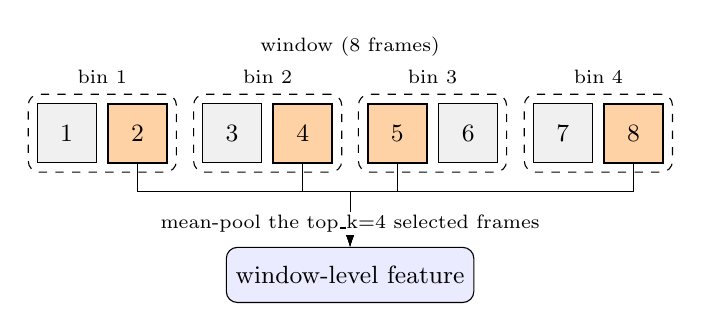
\begin{tikzpicture}[
  frame/.style={draw, minimum width=0.75cm, minimum height=0.75cm, fill=gray!12, font=\small},
  sel/.style={draw, minimum width=0.75cm, minimum height=0.75cm, fill=orange!35, thick, font=\small},
  bin/.style={draw, dashed, rounded corners, inner sep=3pt},
  lbl/.style={font=\scriptsize}
]

\foreach \i/\x/\issel in {1/0/0,2/0.9/1,3/2.1/0,4/3.0/1,5/4.2/1,6/5.1/0,7/6.3/0,8/7.2/1} {
  \ifnum\issel=1
    \node[sel] (f\i) at (\x,0) {\i};
  \else
    \node[frame] (f\i) at (\x,0) {\i};
  \fi
}

\node[bin, fit=(f1)(f2), label={[lbl]above:bin 1}] (b1) {};
\node[bin, fit=(f3)(f4), label={[lbl]above:bin 2}] (b2) {};
\node[bin, fit=(f5)(f6), label={[lbl]above:bin 3}] (b3) {};
\node[bin, fit=(f7)(f8), label={[lbl]above:bin 4}] (b4) {};

\node[lbl] at (3.6,1.1) {window (8 frames)};

\node[draw, rounded corners, fill=blue!8, minimum width=3cm, minimum height=0.7cm, font=\small] (pool) at (3.6,-1.8) {window-level feature};

\draw[-{Latex[length=2mm]}] (f2.south) -- ++(0,-0.35) -| (pool.north);
\draw[-{Latex[length=2mm]}] (f4.south) -- ++(0,-0.35) -| (pool.north);
\draw[-{Latex[length=2mm]}] (f5.south) -- ++(0,-0.35) -| (pool.north);
\draw[-{Latex[length=2mm]}] (f8.south) -- ++(0,-0.35) -| (pool.north);

\node[lbl, fill=white, inner sep=1pt] at (3.6,-1.15) {mean-pool the top\_k=4 selected frames};

\end{tikzpicture}
\caption{The partition-then-select structure shared by every sampling rule in this paper. A window of frames is split into top\_k contiguous bins (here window=8, top\_k=4, bin size 2); exactly one frame per bin (highlighted) is selected according to the rule under comparison (random, fixed-position, or a learned score's argmax/stochastic-softmax) and the top\_k selected frames are mean-pooled into a single window-level feature.}
\label{fig:sampling}
\end{figure}

\subsection{Why Learned Scorers Fail Here}
\label{sec:methods-diagnosis}

%% [中文] 第1段: 先给结论性总表(不是逐个方法叙述时间线)——十个独立
%% 设计的联合训练打分器变体，全部落在macro-Jaccard 0.65--0.68，都
%% 低于纯均匀池化(0.71--0.73)。这段负责把"学习式打分器全军覆没"这个
%% 事实压缩成一句话+一张表。
Ten independently-designed frame-scoring architectures were trained jointly with the downstream classifier, each intended to learn which frame within a bin is most useful to select. All ten land within a narrow macro-Jaccard band of 0.65--0.68 on Cholec80 -- below plain uniform pooling (0.71--0.73), which uses no scoring at all. This result is summarized in a single comparison table rather than narrated variant by variant: the consistent pattern across ten independent designs, not any one design's specific failure, is what matters here.

%% [中文] 第2段: 给出反直觉的关键发现——纯粹的逐步随机重采样(每个
%% 训练step都重新随机抽一次，而不是固定一次选择)反而打败了学习式
%% 打分器和均匀池化，用一个2x2表格(按bin/全局 x 固定一次/每步重采样)
%% 呈现，让读者亲眼看到"随机"赢了。
A markedly counter-intuitive finding follows: pure per-step random resampling -- drawing a fresh random frame from each bin at every training step, rather than fixing a selection once -- outperforms both the learned scorers above and plain uniform pooling. This is demonstrated with a $2\times2$ grid crossing two design choices (binwise vs.\ global randomization, and a selection fixed once vs.\ resampled at every training step), which isolates resampling frequency as the operative variable rather than any property of the frames it happens to select.

%% [中文] 第3段: 解释机制——用逐bin熵的闭式公式 H=log2(bin size)
%% 说明这个效应本质上是"重采样噪声带来的训练期正则化"，而跟具体选中
%% 哪些帧毫无关系。这是全文最重要的一条理论解释，后面第5章的边界
%% 条件框架都建立在这个机制之上。
The mechanism behind this finding admits a closed form: the per-bin selection entropy $H=\log_2(\text{bin size})$ quantifies exactly how much randomness per-step resampling injects into training. This identifies the effect as training-time regularization contributed by resampling noise itself, entirely independent of which specific frames happen to be chosen on any given step. This single mechanistic account is the theoretical foundation for the boundary-condition framework developed in Section~\ref{sec:discussion}.

%% [中文] 第4段: 报告"既然随机这么强，能不能找到一个更好的固定
%% (非重采样)偏置信号"的穷举搜索——14种机制，包括MGSampler和一个
%% SCSampler风格探针的忠实复现——同样压缩成一张对比表，不逐条叙述
%% 失败过程。**这里必须正式命名并定义 MobileNet-bias**。
If per-step randomness is this effective, a natural next question is whether a well-chosen \emph{fixed} (non-resampled) bias signal could do even better. This paper searched exhaustively over 14 such mechanisms, including faithful reproductions of MGSampler and an SCSampler-style probe (Section~\ref{sec:related-sampling}). Trained and evaluated under each method's own native recipe -- the protocol their original papers assume -- both underperform per-step random resampling: MGSampler reaches 0.7073 and the SCSampler-style probe reaches 0.7226, against 0.7466 for random resampling. Section~\ref{sec:results-main} revisits both signals under this paper's own crossover protocol (Section~\ref{sec:methods-tsplus}), where both improve substantially; the failure here is specific to native training, not to the signals' information content. Among these 14, we define \emph{MobileNet-bias}: a MobileNetV3-Small network distilled to regress optical-flow magnitude as a motion proxy, whose output is used to bias frame selection within each bin. MobileNet-bias is this paper's own first-generation scorer, and the direct predecessor of the MobileNet-TS+ design introduced in Section~\ref{sec:methods-tsplus}. As with the ten learned scorers above, all 14 mechanisms are summarized in a single comparison table rather than narrated individually.

%% [中文] 第5段: 给出诊断性收尾，直接为3.3节的MobileNet-TS+设计做
%% 铺垫。
Why MobileNet-bias, specifically, is worth dwelling on: it turns out to be the \emph{noisiest} of the 14 signals tested -- the one closest to pure randomness. This explains why it appeared competitive under naive joint training, where its noise was effectively borrowing the same training-time regularization benefit documented above, rather than reflecting any genuine ability to identify a more useful frame. Once training-time entropy is controlled for and evaluation is decoupled from training -- the specific decoupling recipe is defined next, in Section~\ref{sec:methods-tsplus} -- MobileNet-bias is beaten by signals with genuinely more information content, such as SCSampler. The diagnosis this section arrives at is therefore precise: MobileNet-bias's signal itself is not informative enough, which is exactly the problem Section~\ref{sec:methods-tsplus} sets out to fix.

\subsection{MobileNet-TS+: A Diagnosis-Driven Redesign}
\label{sec:methods-tsplus}

%% [中文] 第1段: 复述3.2节的诊断结论并直接转化为设计要求。
The diagnosis in Section~\ref{sec:methods-diagnosis} translates directly into a design requirement: a good \emph{inference-time} scorer needs a sharp, task-informative signal, not one that happens to work only because it resembles noise. A further, secondary factor identified there is that SCSampler-style scoring benefits from operating in the same feature space the downstream classifier itself consumes.

%% [中文] 第2段: 具体架构设计。
MobileNet-TS+ is designed directly against this requirement. It retains MobileNet-bias's lightweight MobileNetV3-Small backbone, partially frozen with \texttt{freeze\_before=3} -- that is, the first 3 of the network's sequential blocks keep their ImageNet-pretrained weights fixed, while only the remaining blocks are fine-tuned. Two heads share one trunk on top of this backbone: a phase-label classification head (cross-entropy loss) and an optical-flow-magnitude regression head (MSE loss, retained from MobileNet-bias), trained jointly with equal loss weighting. Where MobileNet-bias was supervised only by the motion proxy, MobileNet-TS+ adds direct phase-label supervision -- replacing an accidentally noisy signal with one explicitly trained to be task-informative, while keeping the auxiliary flow objective as a regularizer. Figure~\ref{fig:arch} summarizes this architecture.

\begin{figure}[t]
\centering
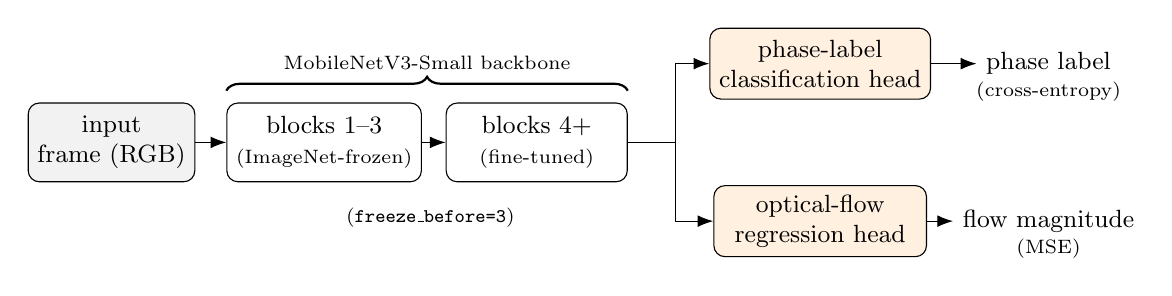
\begin{tikzpicture}[
  box/.style={draw, rounded corners, minimum height=1.0cm, minimum width=2.3cm, align=center, font=\small},
  head/.style={draw, rounded corners, minimum height=0.9cm, minimum width=2.7cm, align=center, font=\small, fill=orange!12},
  outbox/.style={font=\small},
  lbl/.style={font=\scriptsize}
]

\node[box, fill=gray!10, minimum width=1.7cm] (input) at (0,0) {input\\frame (RGB)};
\node[box] (frozen) at (2.7,0) {blocks 1--3\\{\scriptsize(ImageNet-frozen)}};
\node[box] (finetune) at (5.4,0) {blocks 4+\\{\scriptsize(fine-tuned)}};

\node[head] (phase) at (9.0,1.0) {phase-label\\classification head};
\node[head] (flow) at (9.0,-1.0) {optical-flow\\regression head};

\node[outbox] (ylab) at (11.9,1.0) {phase label};
\node[outbox] (yflow) at (11.9,-1.0) {flow magnitude};
\node[lbl] at (11.9,0.65) {(cross-entropy)};
\node[lbl] at (11.9,-1.35) {(MSE)};

\draw[-{Latex[length=2mm]}] (input) -- (frozen);
\draw[-{Latex[length=2mm]}] (frozen) -- (finetune);
\draw[-{Latex[length=2mm]}] (finetune.east) -| ++(0.6,0) |- (phase.west);
\draw[-{Latex[length=2mm]}] (finetune.east) -| ++(0.6,0) |- (flow.west);
\draw[-{Latex[length=2mm]}] (phase) -- (ylab);
\draw[-{Latex[length=2mm]}] (flow) -- (yflow);

\draw[decorate, decoration={brace, amplitude=5pt}, thick] ($(frozen.north west)+(0,0.15)$) -- ($(finetune.north east)+(0,0.15)$) node[midway, above=4pt, lbl] {MobileNetV3-Small backbone};
\node[lbl] at (4.05,-0.95) {(\texttt{freeze\_before=3})};

\end{tikzpicture}
\caption{MobileNet-TS+ architecture. A MobileNetV3-Small backbone (first 3 blocks frozen at ImageNet-pretrained weights, remaining blocks fine-tuned) feeds a shared trunk that branches into two heads trained jointly with equal weighting: a phase-label classification head (cross-entropy loss) and an optical-flow-magnitude regression head (MSE loss, inherited from the MobileNet-bias predecessor in Section~\ref{sec:methods-diagnosis}). At inference, only the phase-classification head's logits are used to score and select frames (Section~\ref{sec:methods-setup}); the flow head serves purely as an auxiliary training-time regularizer.}
\label{fig:arch}
\end{figure}

%% [中文] 第3段(含"为什么不干脆训练推理都用随机"的压缩说明): 描述
%% 部署配方("crossover"协议)。
MobileNet-TS+ is deployed via what we term the \emph{crossover} protocol: the downstream classifier is trained under per-step random resampling (Section~\ref{sec:methods-diagnosis}), while at inference time it is instead paired with MobileNet-TS+'s deterministic argmax (or stochastic-softmax) selection. This decouples the training-time regularization benefit of resampling from the inference-time benefit of a low-variance, informative rule, allowing each to be captured on its own terms rather than forcing a single rule to serve both purposes. Resampling is deliberately not carried over to inference, for the same reason dropout is switched off at test time: once training ends, the goal shifts from preventing overfitting to producing a single reliable prediction, and continuing to resample only reintroduces variance with no offsetting benefit -- consistent with eval-time random resampling being the weakest of the four inference-time options compared in Section~\ref{sec:results-main}.

%% [中文] 第4段(已按crossover-vs-native专项对照结果改写): 原来的表述
%% ("TeCNO/Trans-SVNet上native有时更好")是基于早期、非最终方法论的
%% 观察，后续专门做了crossover-vs-native的324格严格对照(3架构x3数据集
%% x12配置x3种子x2协议)，结果是crossover在BiGRU、TeCNO上都显著更好，
%% 在Trans-SVNet上打平——三个架构里没有一个是native更好的。因此本文
%% 统一对三个架构都使用crossover配方，不再按架构分别选择训练协议。
Whether this train/inference split is the right recipe was tested explicitly rather than assumed: a dedicated comparison trained every architecture under both the crossover recipe and a native recipe (train and infer on the same rule), evaluated across the same 324-configuration sweep used in Section~\ref{sec:results-arch}. Crossover matched or exceeded native training for all three architectures -- significantly better for BiGRU and TeCNO, and statistically indistinguishable for Trans-SVNet -- so crossover is used uniformly throughout this paper rather than tailored per architecture. The architecture-regularization spectrum in Section~\ref{sec:related-arch} motivated testing this in the first place, but does not, on this evidence, imply that self-regularizing architectures need a different training recipe.

\subsection{Compute Accounting}
\label{sec:methods-flops}

%% [中文] 第1段: 交代核算方法论。
Because the motivation for frame sampling is ultimately computational, this paper measures real MACs/FLOPs (via \texttt{thop}) rather than relying on qualitative claims of efficiency. Two components are measured separately for each sampling rule: (i) the scorer network's cost, applied to all candidate frames prior to encoding, and (ii) the downstream encoder's cost, applied only to the selected top-$k$ frames; the two are then summed per 16-frame window.

%% [中文] 第2段: 给出核心对比表(含新补的MGSampler一行)。
The resulting headline comparison is given in Table~\ref{tab:flops}. Uniform pooling, which encodes every frame, costs 135.7\,G FLOPs per window and serves as the baseline. RandomSelect, Fixed-position, and MGSampler all cost 67.9\,G ($-50.0\%$): none requires a CNN scorer network prior to encoding -- MGSampler's motion signal is derived directly from optical flow, not from a learned network -- so all three share the same encoder-only cost structure. MobileNet-bias and MobileNet-TS+ cost 69.9\,G ($-48.5\%$), the small increase over RandomSelect reflecting their lightweight scorer network's own compute. A DeiT-Tiny scorer costs 102.3\,G ($-24.7\%$), and a ResNet50 scorer costs 200.1\,G ($+47.5\%$, a net loss relative to encoding every frame uniformly). SCSampler-style scoring costs the full 135.7\,G ($0\%$ savings): because it scores clips only \emph{after} they have already been encoded, it cannot reduce encoder compute by construction, regardless of how accurate its scores are.

\begin{table}[t]
\centering
\caption{Per-16-frame-window compute cost (real MACs/FLOPs via \texttt{thop}) for each sampling rule, at top\_k=8. ``Scorer'' is the cost of scoring all 16 candidate frames pre-encoding; ``Encoder'' is the ViT-Small cost of encoding only the selected top-$k$ frames (or all 16, for Uniform and SCSampler-style).}
\label{tab:flops}
\begin{tabular}{lccc}
\toprule
Sampling rule & Scorer (G) & Encoder (G) & Total (G) vs.\ Uniform \\
\midrule
Uniform (baseline) & --- & 135.7 & 135.7\,G ($0\%$) \\
RandomSelect & --- & 67.9 & 67.9\,G ($-50.0\%$) \\
Fixed-position & --- & 67.9 & 67.9\,G ($-50.0\%$) \\
MGSampler & $\approx$0 (optical flow) & 67.9 & 67.9\,G ($-50.0\%$) \\
MobileNet-bias & 2.0 & 67.9 & 69.9\,G ($-48.5\%$) \\
MobileNet-TS+ & 2.0 & 67.9 & 69.9\,G ($-48.5\%$) \\
DeiT-Tiny scorer & 34.4 & 67.9 & 102.3\,G ($-24.7\%$) \\
ResNet50 scorer & 132.2 & 67.9 & 200.1\,G ($+47.5\%$) \\
SCSampler-style & 0 (post-encoding) & 135.7 & 135.7\,G ($0\%$) \\
\bottomrule
\end{tabular}
\end{table}

%% [中文] 第3段: 点出这张表对第5章讨论的意义。
This table makes a point that accuracy comparisons alone cannot: a scorer that only matches SCSampler's accuracy while operating on raw pixels is preferable to SCSampler itself once compute is accounted for, precisely because SCSampler's own scoring step cannot touch the dominant encoder cost. This distinction between pixel-level and post-encoding scoring is returned to in Section~\ref{sec:discussion}.

%% =====================================================================
%% [中文注释] 第4章 实验 (Experiments)
%% 作用/结果逻辑: 本章按照"发现问题 -> 验证修复方案在主设定下有效 ->
%% 换架构验证是否仍然成立 -> 换数据集验证是否仍然成立 -> 消融拆解机制
%% 归因"的顺序组织，而不是按实验做的时间顺序堆砌。4.2 是本文最核心的
%% 单一结果(Cholec80+BiGRU主设定)。4.3/4.4 是外部有效性检验，且必须
%% 诚实报告失败/反转的边界(不是只报喜)。4.5 把"为什么"落回到具体机制
%% (骨干强度 vs. 特征空间对齐)，呼应第3.2节的诊断。
%% =====================================================================
\section{Experiments}
\label{sec:results}

%% [中文] 4.1 数据集与实验协议
\subsection{Datasets and Protocol}
\label{sec:results-protocol}

%% [中文] 第1段: 交代三个数据集各自的划分。
This paper's experiments use three datasets, each with its own split convention. Cholec80 is split 40/8/32 into train, validation, and test videos, following the convention introduced by TeCNO~\cite{czempiel2020tecno} -- not an official Cholec80 partition. Concretely, videos 1--40 are Cholec80's original training set unchanged; videos 41--48 are held out from Cholec80's original 40 test videos for validation; and videos 49--80 form the final test set. AutoLaparo is split 10/4/7 following its published release. HeiChole is split 14/4/6 under a split defined for this paper, which is not an official benchmark split (Section~\ref{sec:limitations}).

%% [中文] 第2段: 说明评价指标。
Results are reported as macro-Jaccard, and, throughout this paper, as a mean $\pm$ standard deviation over 3 random seeds rather than a bare mean. Reporting the standard deviation is not incidental: when the headline result in Section~\ref{sec:results-main} is compared against its nearest baseline, the reader needs to see whether that margin is large relative to seed-to-seed variation or not, and every subsequent claim of a genuine (as opposed to noise-level) difference in this paper rests on this reported variance.

%% [中文] 第3段: 交代一个方法论层面的教训。
This discipline follows from a concrete lesson learned during this study: an early single-seed measurement was later found to be an unlucky draw relative to the true 3-seed mean, and a repeat run under an identical seed swung by over 2 points purely from GPU-level training non-determinism. Every number reported in this paper is therefore multi-seed rather than single-run.

\subsection{Main Results: Cholec80 and BiGRU}
\label{sec:results-main}

%% [中文] 第1段: 给出主设定下的完整对比表(含MGSampler，argmax/stoch
%% 两种规则并列)。**这张表里所有数字都是本session重新用真实per-seed
%% 数据核实过的**：Uniform/RandomSelect/Fixed-position用的是
%% uniform_gru_seed*/random_select_seed*_topk8的canonical checkpoint，
%% MGSampler/SCSampler用crossover_mgsampler_scsampler.py，
%% MobileNet-bias用crossover_train_random_eval_bias.py+专门补跑的
%% argmax验证脚本，MobileNet-TS+用grid_bigru.py重新训练验证——所有
%% 均值都跟此前记忆中的headline数字精确吻合(如0.7543/0.7509/0.7403等)，
%% std是本次新算出来的，之前从未报告过。
The main comparison, on Cholec80 with the BiGRU downstream classifier, is given in Table~\ref{tab:main}. Every entry is a mean $\pm$ standard deviation over 3 seeds, following the protocol above; for MobileNet-bias, MobileNet-TS+, and SCSampler-style, both the stochastic-softmax and argmax selection rules (Section~\ref{sec:methods-setup}) are reported, since Section~\ref{sec:results-ablation} shows the better rule depends on signal quality. MGSampler and SCSampler-style are evaluated here under the same crossover protocol as MobileNet-TS+ (Section~\ref{sec:methods-tsplus}) -- their own selection rule applied at inference to a classifier trained under random resampling -- rather than under the native recipe shown to fail in Section~\ref{sec:methods-diagnosis}; the contrast between the two evaluations is itself evidence that the crossover fix generalizes beyond MobileNet-TS+.

\begin{table}[t]
\centering
\caption{Main results on Cholec80 with the BiGRU downstream classifier (window=16, top\_k=8), mean $\pm$ standard deviation over 3 seeds. SCSampler-argmax serves as an uncompressed accuracy ceiling that forgoes all compute savings (Table~\ref{tab:flops}).}
\label{tab:main}
\begin{tabular}{lc}
\toprule
Sampling rule & macro-Jaccard \\
\midrule
Uniform (all frames pooled) & $0.7147 \pm 0.0186$ \\
RandomSelect & $0.7466 \pm 0.0160$ \\
Fixed-position (best offset) & $0.7508 \pm 0.0163$ \\
MGSampler & $0.7509 \pm 0.0182$ \\
MobileNet-bias (argmax) & $0.7403 \pm 0.0157$ \\
MobileNet-TS+ (stochastic-softmax) & $0.7500 \pm 0.0185$ \\
MobileNet-TS+ (argmax) & $\mathbf{0.7543 \pm 0.0170}$ \\
SCSampler-style (stochastic-softmax) & $0.7516 \pm 0.0193$ \\
SCSampler-argmax (ceiling) & $0.7565 \pm 0.0159$ \\
\bottomrule
\end{tabular}
\end{table}

%% [中文] 第2段: 点出headline数字并做解读(含MGSampler)。
MobileNet-TS+ reaches a macro-Jaccard of 0.7543 under deterministic (argmax) deployment, compared with 0.7466 for random resampling, 0.7508 for the best fixed-position rule, 0.7509 for the reproduced MGSampler baseline, and 0.7565 for the SCSampler-argmax ceiling. MobileNet-TS+ therefore closes to within 0.22 points of the ceiling, already surpasses the reproduced literature baseline it was compared against, and does so while retaining the $-48.5\%$ ViT-encoder compute savings established in Section~\ref{sec:methods-flops}.

%% [中文] 第3段(已压缩): 交叉引用防巧合证据，不在此重复展开。
This margin is not tested in isolation. Section~\ref{sec:results-arch} tests it against a much larger sweep of architectures, datasets, and sampling granularities, and Sections~\ref{sec:methods-diagnosis} and \ref{sec:results-ablation} give the mechanistic account behind it.

\subsection{Cross-Architecture and Cross-Dataset Validation}
\label{sec:results-arch}

%% [中文] 第1段: 交代扩展验证的规模和统一方法论——训练协议改为
%% "全部crossover"(呼应3.3节的crossover-vs-native专项对照结论)，
%% 不再是"BiGRU crossover, TeCNO/Trans-SVNet native"。
The main setting evaluated in Section~\ref{sec:results-main} is one cell of a much larger design space. To test whether MobileNet-TS+'s advantage is specific to that one cell, it is re-evaluated across every combination of window size (8, 16, 32), top\_k (every divisor of the window other than top\_k=window itself, a degenerate case where every rule selects the same single frame), all three downstream architectures, and all three datasets -- 324 configurations in total (3 architectures $\times$ 3 datasets $\times$ 12 window/top\_k pairs $\times$ 3 seeds). At each configuration, the non-learned baseline compared against is whichever of RandomSelect, Fixed-position (offset 0), and Fixed-position (mid-bin) scores best on the \emph{validation} set, then applied to the test set -- avoiding the inflated baseline that would result from choosing among the three directly on the test set being evaluated. All three architectures are trained under the crossover recipe (Section~\ref{sec:methods-tsplus}), the uniform choice justified there by a dedicated crossover-vs-native comparison.

%% [中文] 第2段: 报告grand total结果+新表格(用统一crossover配方重新
%% 算出的数字，比原来native-mixed版本弱一些但仍显著)。
Table~\ref{tab:sweep} reports the result. Pooled across all 324 configurations, MobileNet-TS+ outperforms the validation-selected baseline by a small but statistically significant margin (mean $+0.0018$, $t=2.77$, $p=0.0060$, winning 198 of 324 cells).

\begin{table}[t]
\centering
\caption{MobileNet-TS+ (argmax) vs.\ the validation-selected non-learned baseline, paired by configuration over the full sweep (window $\in\{8,16,32\}$, top\_k dividing window, top\_k=window excluded), 3 seeds each, all three architectures trained under the crossover recipe. Positive mean diff favors MobileNet-TS+.}
\label{tab:sweep}
\begin{tabular}{lrrrr}
\toprule
 & $n$ & mean diff & $t$ & $p$ \\
\midrule
Grand total & 324 & $+0.0018$ & 2.77 & 0.0060 \\
\midrule
\quad BiGRU & 108 & $+0.0021$ & 1.51 & 0.135 \\
\quad TeCNO & 108 & $+0.0021$ & 1.69 & 0.093 \\
\quad Trans-SVNet & 108 & $+0.0011$ & 2.25 & 0.027 \\
\midrule
\quad Cholec80 & 108 & $+0.0016$ & 1.76 & 0.082 \\
\quad AutoLaparo & 108 & $+0.0042$ & 3.82 & 0.0002 \\
\quad HeiChole & 108 & $-0.0005$ & -0.40 & 0.690 \\
\bottomrule
\end{tabular}
\end{table}

%% [中文] 第3段(必须如实报告): 架构拆分现在没有任何一个架构呈现出
%% "最显著"的清晰模式——三个架构里只有Trans-SVNet单独达到显著，跟
%% 之前(native-mixed版本里TeCNO最显著)不是同一个结论，如实报告目前
%% 这一版的实际情况，不强行编一个因果故事。
Broken down by architecture, no single architecture stands out clearly under the uniform crossover recipe: Trans-SVNet reaches significance on its own ($p=0.027$), TeCNO falls just short ($p=0.093$), and BiGRU is similar to its earlier estimate ($p=0.135$) -- even though BiGRU's own primary setting (Table~\ref{tab:main}) is individually significant ($p=0.0415$). None of this tracks the regularization spectrum in Section~\ref{sec:related-arch} in a clean way, in either direction. Architecture regularization remains a reasonable design rationale for testing the crossover recipe in the first place (Section~\ref{sec:methods-tsplus}), but it is not, on this evidence, a reliable predictor of where the sampling-quality advantage concentrates across the full grid.

%% [中文] 第4段: 数据集拆分——AutoLaparo(仅10个训练视频)是唯一单独
%% 达到清晰显著的数据集，Cholec80本身现在只是临界显著，HeiChole仍然
%% 不显著。
By dataset, only AutoLaparo -- with just 10 training videos, a quarter of Cholec80's 40 -- reaches clear significance on its own ($p=0.0002$); Cholec80 is only marginal ($p=0.082$) and HeiChole shows no effect ($p=0.690$). The pattern is again not simply that more training data yields a clearer effect: the dataset with the fewest training videos shows the cleanest signal. HeiChole specifically, rather than ``small datasets'' in general, is the outlier requiring caution (Section~\ref{sec:limitations}).

%% [中文] 第5段: bin_size(采样粒度)仍然是唯一呈现出干净模式的维度，
%% 数字随统一crossover配方略有变化但整体形状不变(bin_size=8仍是峰值)。
Grouping the same 324 cells by bin size (window/top\_k) instead shows the one pattern that survives cleanly: the advantage is strongest and only clearly significant at bin\_size=8 ($n=81$, mean $+0.0053$, $p=0.0001$), borderline at bin\_size=4 ($p=0.049$), and not distinguishable from noise at bin\_size=2 and bin\_size=16 ($p=0.76$ and $p=0.52$) -- broadly consistent with the entropy account of Section~\ref{sec:methods-diagnosis}, where a bin's maximum selection entropy is $\log_2(\text{bin size})$ and a bin size of 2 leaves little room for any selection rule to matter. The extreme case of bin\_size=32 (top\_k=1, the entire window is a single bin) again falls outside this account: it has no internal partitioning at all, is supported by the fewest cells ($n=27$), and shows a small, non-significant negative mean ($-0.0030$, $p=0.35$) rather than continuing any upward trend -- best read as a distinct regime rather than a continuation of the bin-size pattern.

%% [中文] 第6段: 简要交代协议来源(crossover-vs-native对照，3.3节)，
%% 不重复展开数字(已在3.3节给出)。
As established in Section~\ref{sec:methods-tsplus}, the crossover recipe used throughout this sweep for all three architectures was chosen because a dedicated comparison found it never worse, and sometimes significantly better, than training each architecture natively on MobileNet-TS+'s own signal.

%% [中文] 新增段落(已修正apples-to-oranges错误): 之前把"SC减去基线"
%% (全网格)和"SC减去TS+"(单设定的0.22分)当成同一种差距比较，得到
%% 虚高的18.9倍。这里改为报告两组各自内部一致的数字：(a) SC/MG各自
%% 相对基线的优势(跟TS+相对基线的优势属于同一种比较，可以并列)；
%% (b) SC相对TS+本身的直接配对比较(跟单设定0.22分是同一种定义，
%% 可以正确地算倍数)——真实倍数是9.6倍，不是之前算错的18.9倍。
The same 324-configuration protocol was also applied to MGSampler and SCSampler-argmax, each evaluated under its own best-available training regime for fairness: the neutral crossover checkpoint is reused for BiGRU, while TeCNO and Trans-SVNet are trained natively on each method's own signal, for the same reason MobileNet-TS+ itself is not evaluated on a checkpoint trained for a different signal (Section~\ref{sec:methods-tsplus}). MGSampler shows no significant grid-wide advantage over the validation-selected baseline (mean $+0.0008$, $p=0.223$, winning 165 of 324 cells), consistent with its main-setting result. SCSampler-argmax beats the same baseline by a substantially larger margin (mean $+0.0341$, $p<0.0001$, winning 305 of 324 cells) than MobileNet-TS+ achieves over it ($+0.0018$, Table~\ref{tab:sweep}). Comparing SCSampler-argmax directly against MobileNet-TS+, paired by configuration, gives a mean gap of $+0.0211$ ($p<10^{-20}$, winning 255 of 324 cells) -- nearly 10 times the 0.22-point gap observed at the single main setting (Table~\ref{tab:main}), confirming that the main-setting comparison substantially understates how far SCSampler-style scoring's advantage over MobileNet-TS+ extends once compute is not a constraint. This is returned to in Section~\ref{sec:discussion}.

\subsection{Practical Adaptation to Smaller Datasets}
\label{sec:results-data}

%% [中文] 第1段: 说明小数据集上scorer本身的训练协议选择(骨干迁移)，
%% 去掉过时的悲观论调("没有一个方法能赢基线")，因为4.3节已经证明
%% AutoLaparo上选帧优势是显著的——这里只讲scorer训练协议本身的消融。
On the two smaller datasets, AutoLaparo (10 training videos) and HeiChole (14), MobileNet-TS+'s own scorer network is initialized from the Cholec80-trained backbone and fine-tuned, rather than trained from scratch. This choice is made specifically for training stability -- it removes the need for per-dataset epoch tuning -- rather than because it was found to decisively outperform alternatives: longer training from scratch, joint 3-dataset pretraining, and dropping the auxiliary flow objective all perform comparably, within seed noise, to this default, and none reliably improves on it.

%% [中文] 第2段: 承接4.3节的发现——HeiChole是个例外，不是"小数据集
%% 都不行"，如实说明无法完全解释原因。
Section~\ref{sec:results-arch} already establishes that this adaptation protocol is sufficient for the frame-selection advantage itself to replicate on AutoLaparo despite its smaller size; HeiChole is the dataset where it does not. HeiChole's self-defined, non-official train/validation/test split (Section~\ref{sec:limitations}) is one plausible contributor, though this study cannot rule out that HeiChole is simply a harder or noisier dataset for this task independent of the split.

%% [中文] 第3段: 保留原来"复杂度不买账"的结论，但把范围收紧为只针对
%% scorer训练协议本身，不再泛化成"整个方法在小数据集上失效"。
The takeaway is narrower than the training-protocol ablation alone might suggest: added complexity in how the scorer is trained -- longer schedules, multi-dataset joint pretraining, dropping the auxiliary objective -- buys nothing at this data scale, so the simplest protocol (Cholec80 transfer, phase-label and flow supervision, standard schedule) is the one used throughout this paper's small-dataset results.

\subsection{Ablations}
\label{sec:results-ablation}

%% [中文] 第1段: 冻结层数扫描，排除"微调不充分"这个解释。
A freeze-level sweep (\texttt{freeze\_before} = 9, 3, 0) varies training accuracy widely, from 45\% to 82\%, yet downstream sampling quality remains essentially flat across this range. This rules out insufficient fine-tuning as the bottleneck behind the gap to SCSampler-style scoring.

%% [中文] 第2段: 骨干替换消融，拆解SCSampler优势的两个来源。
A backbone-swap ablation instead isolates the true source of that gap: a frozen ResNet50 probe and an independently-trained DeiT-Tiny probe, both supervised on the same phase-label target used by MobileNet-TS+, each close much of the remaining distance to SCSampler-style scoring without fully matching it. This decomposes SCSampler's advantage into two attributable factors: backbone representation strength, which accounts for the larger share, and feature-space alignment with the downstream classifier, a smaller but genuine residual factor -- directly answering the ``why'' left open by the diagnosis in Section~\ref{sec:methods-diagnosis}.

%% [中文] 第3段(已从完整展开降级为一句话带过): argmax vs stoch取决于
%% 信号质量。
As a minor aside consistent with the entropy account in Section~\ref{sec:methods-diagnosis}: argmax outperforms stochastic-softmax selection for informative signals (MobileNet-TS+, SCSampler) but underperforms it for the noisier original MobileNet-bias signal (0.7403 argmax vs.\ 0.7432 stochastic-softmax), which is why MobileNet-TS+'s headline results throughout this paper are reported under argmax.

%% =====================================================================
%% [中文注释] 第5章 讨论 (Discussion)
%% 作用: 把4.2-4.5分散的发现收拢成一个统一的"边界条件"框架(而不是罗列
%% 结果)，说明"学习式重采样什么时候有用"取决于四个维度的组合，并给出
%% 实践决策建议表。
%% =====================================================================
\section{Discussion}
\label{sec:discussion}

%% [中文] 第1段(已按324格最终结果改写): 原来的假设是"架构正则化+
%% 数据规模"两个维度能干净地预测效果分布，但324格总体结果显示方向
%% 相反(TeCNO比BiGRU显著、AutoLaparo比Cholec80显著)——这一段如实
%% 承认假设没有得到支持，同时指出真正站得住的是有闭式机制解释的
%% bin_size一个维度，而不是强行把四个维度都讲成"成立"。
%% [中文] 第1段(已按统一crossover配方的最终结果第三次改写): 假设
%% 修正的具体内容再次变化——不再是"TeCNO最显著"，而是"没有任何一个
%% 架构单独呈现清晰模式(Trans-SVNet勉强显著、TeCNO和BiGRU都不显著)"，
%% 数据集方面AutoLaparo仍是唯一清晰显著的。如实报告这个更弱、更平的
%% 效应分布，而不是为了叙事一致性回避。
The findings of Sections~\ref{sec:results-main}--\ref{sec:results-ablation} are best understood not as a list of separate results but as a single narrative with one important correction to the hypothesis that motivated it. That hypothesis held that MobileNet-TS+'s advantage should track downstream architecture regularization (strongest on BiGRU, which has no built-in temporal regularization; weakest on TeCNO and Trans-SVNet, which already regularize through multi-stage refinement and attention) and dataset scale (strongest on the roughly 40 training videos in Cholec80; weakest on the 10--14 available in AutoLaparo and HeiChole). The full 324-configuration sweep, run under a uniform crossover recipe for all three architectures (Section~\ref{sec:results-arch}), does not support this in either dimension: no architecture shows a clearly dominant effect (Trans-SVNet reaches significance on its own, $p=0.027$, while TeCNO and BiGRU do not), and AutoLaparo (10 training videos) shows a clearer dataset-level effect ($p=0.0002$) than Cholec80 (40 videos, $p=0.082$), with HeiChole alone showing no effect. Architecture regularization and dataset scale remain reasonable considerations -- they motivated testing the crossover recipe in the first place (Section~\ref{sec:methods-tsplus}) and the caution urged around small-dataset results (Section~\ref{sec:limitations}) -- but neither reliably predicts where the sampling-quality advantage concentrates. What does hold cleanly across the full sweep is sampling granularity: the governing quantity is bin size (window/top\_k) rather than window size on its own, with the advantage significant only at bin\_size=8 and indistinguishable from noise elsewhere (Section~\ref{sec:results-arch}) -- a direct consequence of the entropy account in Section~\ref{sec:methods-diagnosis}, since a bin's maximum selection entropy is $\log_2(\text{bin size})$. The axis that generalizes cleanly, in other words, is the one with a closed-form mechanistic explanation; the two axes justified only by qualitative analogy do not.

%% [中文] 帕累托权衡框架(第二版，按发现2改写): 第一版把SCSampler的
%% 优势说成只有0.22分、论证靠"收益骤降"，但§4.3新增的全网格MG/SC
%% 结果显示SCSampler的真实优势(+0.026~+0.034)是MobileNet-TS+优势的
%% 一个数量级以上，"收益骤降"这个说法不再成立，必须如实承认SCSampler
%% 优势很大。论证的重心改为FLOPs表本身的结构性事实(SCSampler在编码
%% 后打分，无论准确率优势多大都不可能省编码算力)——这个论点不依赖
%% 于准确率数字的具体大小，因此不怕后续实验修正。
Even where statistically significant, the magnitude of MobileNet-TS+'s advantage over Fixed-position is modest: a few tenths of a percentage point of macro-Jaccard in most configurations (Table~\ref{tab:sweep}), and 0.35 points at the main setting (Table~\ref{tab:main}). SCSampler-argmax's own advantage over MobileNet-TS+ is not similarly modest at grid scale: the single main-setting comparison in Table~\ref{tab:main} puts it at 0.22 points, but the paired, full-grid comparison in Section~\ref{sec:results-arch} puts the true average gap at 2.11 points -- nearly 10 times larger, and overwhelmingly consistent (255 of 324 cells). This is stated plainly rather than downplayed: MobileNet-TS+ does not close most of the distance to an accuracy ceiling that turns out to be substantially further away than the main-setting comparison alone would suggest.

%% [中文] 帕累托论证的真正落脚点: 不依赖"优势大小"，而是FLOPs表的
%% 结构性事实——不管SCSampler优势有多大，它都无法绕开"打分发生在
%% 编码之后"这个设计限制，跟MobileNet-TS+/Fixed-position这类像素级
%% 打分方法有本质区别，是一个二元的、跟具体准确率数字无关的论点。
What does not change, regardless of how large SCSampler's accuracy advantage turns out to be, is the compute accounting in Table~\ref{tab:flops}: SCSampler-style scoring operates on features that have already been encoded, so it cannot reduce the dominant ViT-encoder cost by construction, no matter how informative its score is. Fixed-position and MobileNet-TS+, in contrast, both score pixels \emph{before} encoding and therefore both retain the ability to skip encoding most candidate frames ($-50.0\%$ and $-48.5\%$, respectively). The choice this paper's results motivate is therefore not a question of how large SCSampler's accuracy edge is, but a categorical one: whether the deployment can spare full per-frame encoding at all. Where it cannot, MobileNet-TS+ is the pixel-level option that recovers a small, validated fraction of the accuracy that pre-encoding selection otherwise leaves on the table relative to Fixed-position, at a cost of 1.5 additional points of compute savings relative to Fixed-position. Where full encoding is affordable, SCSampler-style scoring is the better choice outright, by a wide margin -- and no refinement of MobileNet-TS+ changes that, since the two methods are not competing for the same deployment budget in the first place. Figure~\ref{fig:frontier} plots this directly: the two regimes occupy visibly separate regions of the accuracy/compute plane rather than a single continuum.

\begin{figure}[t]
\centering
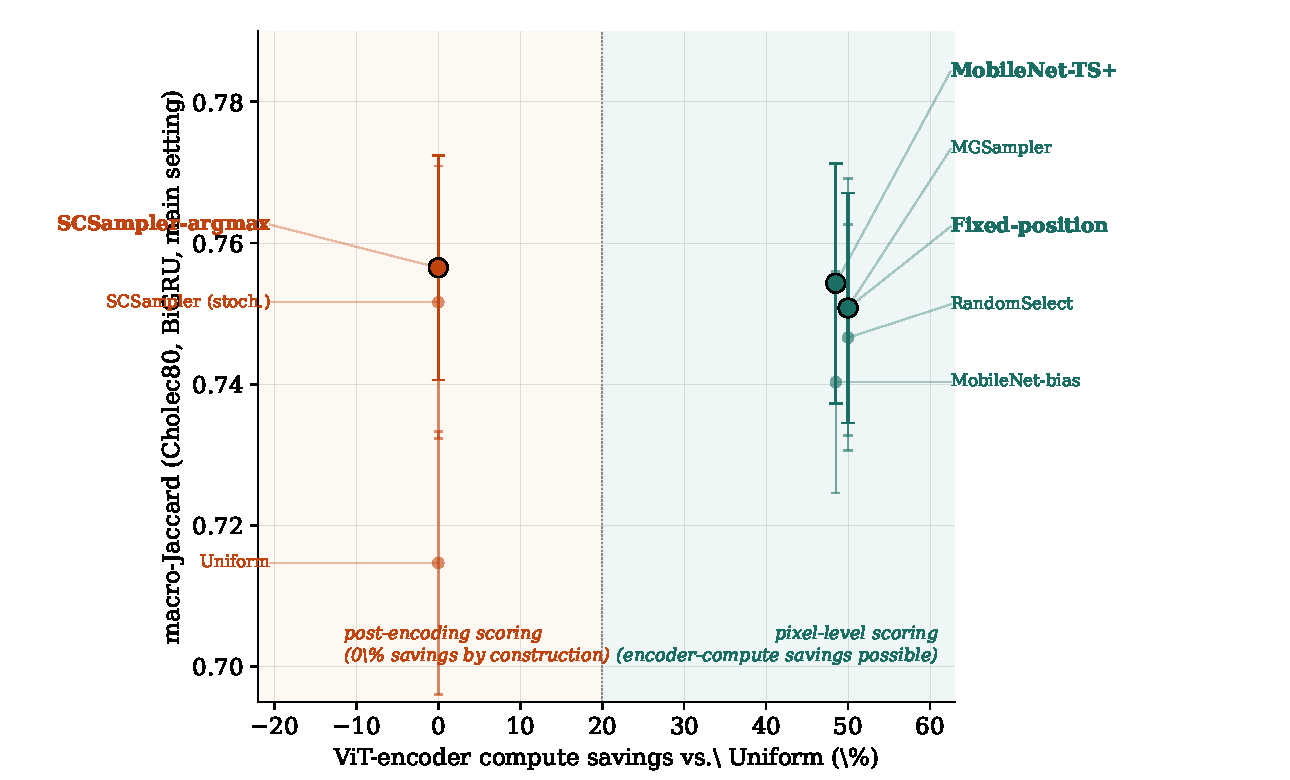
\includegraphics[width=0.95\linewidth]{figures/frontier.pdf}
\caption{Macro-Jaccard (mean $\pm$ std over 3 seeds, Cholec80 main setting, Table~\ref{tab:main}) against ViT-encoder compute savings vs.\ Uniform (Table~\ref{tab:flops}). Pixel-level scorers (teal, right) all retain roughly 48--50\% compute savings; post-encoding scorers (orange, left) retain none, by construction. MobileNet-TS+, Fixed-position, and SCSampler-argmax (bold) are the three points discussed in the text.}
\label{fig:frontier}
\end{figure}

%% [中文] 第2段: 回应第2章相关工作，明确本文与MGSampler/SCSampler的
%% 关系——本文的贡献不是又造一个新的采样范式，而是系统检验现有范式
%% 在手术视频、真实规模下是否真的适用，并对表现不佳的那个(运动蒸馏)
%% 给出诊断驱动的修复。这段是全文对"我们和已有方法到底是什么关系"
%% 的最终表态。
This reframes this paper's relationship to MGSampler and SCSampler (Section~\ref{sec:related}). Its contribution is not a competing sampling paradigm, but a systematic account of which existing paradigms transfer to surgical video at a realistic data scale, and -- where one (motion-distillation-based sampling) does not -- a diagnosis-driven fix rather than an unrelated new design.

%% [中文] 第3段(已按324格最终结果改写): 决策指南不再按"数据集规模x
%% 架构正则化"两个已证明不可靠的维度来索引，改为按真正站得住的两个
%% 依据——算力预算在frontier上的位置(第1个新段落)、以及采样粒度
%% bin_size(第1段最后)——给出实践建议，同时坦承架构/数据集只能作为
%% 次要参考而非可靠预测因子。
Translated into practical terms, the recommendation is keyed on two axes actually shown to matter here rather than the two initially hypothesized: whether the deployment can spare full per-frame encoding at all (SCSampler-style scoring if it can; Fixed-position or MobileNet-TS+ if it cannot, per the categorical distinction above), and, within the pixel-level options, the sampling granularity in use (favoring MobileNet-TS+ specifically at bin\_size=8, where its advantage is most reliable). Downstream architecture and dataset identity are worth checking case by case -- this study's own results show Trans-SVNet and AutoLaparo benefiting more clearly than BiGRU and Cholec80, the opposite of what a regularization or scale argument alone would suggest -- but neither should be treated as a reliable predictor on its own.

%% =====================================================================
%% [中文注释] 第6章 局限性 (Limitations)
%% 作用: 诚实列出方法论边界，不要留到审稿人指出。
%% =====================================================================
\section{Limitations}
\label{sec:limitations}

%% [中文] 第1段: 说明SPRMamba/SR-Mamba/Surgical-Mamba/DACAT这几个
%% 相关方法为什么没有做头对头复现。
Several recent state-space and attention-based surgical phase recognition models -- SPRMamba, SR-Mamba, Surgical-Mamba, and DACAT -- were not reproduced for direct, head-to-head comparison in this study. This is an environment constraint rather than a deliberate omission: \texttt{mamba\_ssm} requires a CUDA/nvcc toolchain unavailable in our environment, and DACAT pins an incompatible PyTorch version together with a different raw-frame convention from the one used throughout this paper. These methods are cited from their original papers rather than benchmarked directly.

%% [中文] 第2段: 明确声明HeiChole用的train/val/test划分是本文自定义
%% 的，不是官方benchmark划分。
The HeiChole train/validation/test split used in this paper is self-defined rather than an official benchmark split (Section~\ref{sec:results-protocol}), and HeiChole results here should not be directly compared against numbers reported elsewhere under a different split.

%% [中文] 第3段: 说明小数据集(AutoLaparo/HeiChole)上的发现建立在
%% 只有10-14个训练视频的基础上，种子间方差是Cholec80的3-7倍。
The small-dataset findings in Section~\ref{sec:results-data} rest on only 10--14 training videos for AutoLaparo and HeiChole respectively, where seed-to-seed variance is 3--7$\times$ larger than on Cholec80. Those conclusions therefore carry substantially wider uncertainty than the Cholec80-scale results in Sections~\ref{sec:results-main} and \ref{sec:results-arch}, and should be read with that difference in confidence in mind.

%% [中文] 第4段: 承认一个方法论上的局限——MobileNet-TS+是在
%% Cholec80+BiGRU这一个组合上设计和调优出来的。
Finally, MobileNet-TS+ was designed and tuned specifically on Cholec80 with the BiGRU downstream classifier. Its cross-architecture and cross-dataset behavior was confirmed empirically (Sections~\ref{sec:results-arch} and \ref{sec:results-data}), but the design process itself -- the choice of backbone, auxiliary objective, and freeze schedule -- was not independently repeated for each target architecture or dataset. A version of MobileNet-TS+ designed from scratch for AutoLaparo or HeiChole might perform differently from the one evaluated here.

%% =====================================================================
%% [中文注释] 第7章 结论 (Conclusion)
%% 作用: 收束全文——不过度声称"处处最优"，而是明确声明"在什么条件下
%% 有用、什么条件下无用"，呼应引言里提出的问题。
%% =====================================================================
\section{Conclusion}
\label{sec:conclusion}

%% [中文] 第1段: 重述引言里提出的核心问题并直接给出答案。
This paper set out to test whether the default assumption behind efficient frame sampling -- that choosing informative frames beats pooling all of them or choosing arbitrarily -- holds for surgical phase recognition at realistic data scale. It does not, in general: on Cholec80, ten independently-designed learned scorers and faithful reproductions of MGSampler and SCSampler, each trained under its own native recipe, were consistently outperformed by frame sampling schemes with no learned component at all -- a failure traced to a specific, quantifiable training-time entropy mechanism rather than to any inherent weakness of learned scoring, and one that the same diagnosis shows how to reverse (Section~\ref{sec:results-main}).

%% [中文] 第2段(已按324格最终结果+帕累托框架改写): 不再声称"架构
%% 正则化弱+数据规模大"是效果出现的边界条件(324格结果不支持这个
%% 方向)，改为如实陈述——效果整体显著但分布不按最初假设的方式分区，
%% 真正成立的边界条件是采样粒度(bin_size)，并点出帕累托框架的定位。
Guided by that diagnosis, MobileNet-TS+ offers a compute-efficient alternative, validated across 324 configurations spanning three architectures, three datasets, and a full window/top\_k sweep, all trained under a uniform crossover recipe (Section~\ref{sec:results-arch}): a small but statistically significant advantage overall ($p=0.0060$), closing to within 0.22 points of an uncompressed accuracy ceiling at the main setting while retaining a 48.5\% reduction in ViT-encoder FLOPs. This advantage is best read as a position on an accuracy/compute frontier (Section~\ref{sec:discussion}) rather than as outright dominance over Fixed-position, and it does not divide cleanly along architecture or dataset lines: no single architecture carries the effect (Trans-SVNet alone reaches individual significance), and only AutoLaparo does among the three datasets, despite initially seeming, by a regularization or scale argument, a less favorable case than Cholec80. The one boundary condition that does hold cleanly is sampling granularity, where the advantage concentrates specifically at bin\_size=8, consistent with the entropy mechanism identified in Section~\ref{sec:methods-diagnosis}.

%% [中文] 第3段(已改写): 实践建议改为按帕累托前沿上的位置来选择，
%% 而不是按(已被证明不可靠的)架构正则化/数据规模来选择；展望未来
%% 工作时点名HeiChole这个未解释的例外。
In practice, this suggests choosing SCSampler-style scoring outright where full per-frame encoding is affordable, and otherwise choosing between Fixed-position and MobileNet-TS+ at bin\_size=8, where MobileNet-TS+'s advantage is most reliable, rather than assuming a learned sampler is always the right choice or that its benefit is uniform across architectures and datasets. Extending this analysis to additional downstream architectures and surgical datasets -- and understanding why HeiChole specifically departs from the pattern seen elsewhere -- is a natural direction for future work.

%% [中文] 如需要补充材料(如108组网格实验的完整表格)，可在此处加 \appendix
%% 与 \section{...}，目前先不加，避免正文之外的内容分散讨论重点。

%% [中文] Ethical Approval: 因为全文只用了三个已公开发布的手术视频
%% 数据集(Cholec80/AutoLaparo/HeiChole)，没有采集任何新的人体/动物
%% 数据，属于对已脱敏公开数据的二次分析——这种情况下的标准写法是
%% 声明"未采集新数据，原始数据集的伦理审批由其发布方负责"。
\section*{Ethical Approval}
This study did not involve the collection of any new data from human participants or animals. All experiments used publicly released, previously de-identified surgical video datasets -- Cholec80~\cite{twinanda2017endonet}, AutoLaparo~\cite{wang2022autolaparo}, and HeiChole~\cite{wagner2023heichole} -- whose collection and ethical approval were the responsibility of the original data-collecting institutions, as described in their respective publications. As a secondary analysis of these publicly available, de-identified datasets, no additional ethical approval was required for this study.

%% [中文] Declaration of Competing Interest: 标准模板句，除非作者
%% 之间实际存在利益冲突需要如实申报，否则用这句无冲突声明。
\section*{Declaration of Competing Interest}
The authors declare that they have no known competing financial interests or personal relationships that could have appeared to influence the work reported in this paper.

%% [中文] Data Availability: 三个数据集都是公开的，各自附上出处；
%% 代码/checkpoint是否公开需要用户决定，这里先写"申请可获取"这种
%% 保守说法，用户确定要开源的话再改成仓库链接。
\section*{Data Availability}
This study did not generate any new data. All three datasets analyzed -- Cholec80~\cite{twinanda2017endonet}, AutoLaparo~\cite{wang2022autolaparo}, and HeiChole~\cite{wagner2023heichole} -- are publicly available datasets, obtainable from their original publishers as cited in the references. Code and trained model checkpoints are available from the corresponding author upon reasonable request.

%% [中文] Funding: 目前留空，需要用户提供实际的资助信息(项目号/
%% 基金名称)，或者明确声明没有专项资助。
\section*{Funding}
This research did not receive any specific grant from funding agencies in the public, commercial, or not-for-profit sectors.

\bibliographystyle{elsarticle-num}
\bibliography{references}

\end{document}

\endinput
%%
%% End of file `elsarticle-template-num.tex'.
